\documentclass[conference]{IEEEtran}
\IEEEoverridecommandlockouts
% The preceding line is only needed to identify funding in the first footnote. If that is unneeded, please comment it out.
\usepackage{cite}
\usepackage{amsmath,amssymb,amsfonts}
\usepackage{algorithmic}
\usepackage{graphicx}
\usepackage{textcomp}
\usepackage{xcolor}
\usepackage{pgfplots}
\usepackage{csvsimple}
\usepackage{tikz}
\usepackage{filecontents}
\usepackage{float}

\def\BibTeX{{\rm B\kern-.05em{\sc i\kern-.025em b}\kern-.08em
    T\kern-.1667em\lower.7ex\hbox{E}\kern-.125emX}}
\begin{document}

\graphicspath{{./figures/}}

\title{Electrogardiograma ECG}

\author{
\IEEEauthorblockN{1\textsuperscript{st} Sergio Carracedo Rodríguez}
\IEEEauthorblockA{\textit{Instrumentación Biomédica} \\
\textit{Universitat Politècnica de València}\\
Valencia, España \\
scarrod@teleco.upv.es}
\and
\IEEEauthorblockN{2\textsuperscript{nd} Jorge Huertas Pastor}
\IEEEauthorblockA{\textit{Instrumentación Biomédica} \\
\textit{Universitat Politècnica de València}\\
Valencia, España \\
jorhuepa@teleco.upv.es}
}

\maketitle

\begin{abstract}
En esta práctica se ha trabajado alrededor del ECG. Caracterizando un dispositivo que realiza esta función y diseñando un programa en LabVIEW capaz de mostrar por pantalla tanto la señal del ECG realizado como las pulsaciones por minuto (ppm) que tiene la persona en cuestión.
\end{abstract}

\section{Introducción}
Esta práctica se ha dividido en dos partes, una de ellas consiste en caracterizar un utilizado para la realización del ECG y posteriormente utilizado para la capatura de la señal mediante la placa NI myRIO y su muestra en el PC.

\section{Amplificador de ECG}
\subsection{Respuesta en frecuencia sin filtro notch}
En la gráfica siguiente se muestra la tensión pico-pico $V_{pp}$ de la señal conforme va variando la frecuencia. En este caso el filtro noctch está \textit{desactivado}.

\begin{figure}[H]
    \begin{tikzpicture}
        \begin{axis}[xmode=log, 
            grid=both,
            xlabel={$f$ (Hz)},
            ylabel={G (dB)}]
        \addplot+[mark size=1pt] table [x=f, y=g, col sep=comma] {g_sinNotch.csv};
        \end{axis}
        \end{tikzpicture}
    \caption{Ganancia sin filtro notch}
    \label{g_sinNotch}
    \end{figure}

En esta gráfica se puede observar la respuesta plana en la banda que estamos observando (desde los 0.5 Hz a los 100 Hz).

\subsection{Respuesta en frecuencia con filtro notch}
En la gráfica siguiente se muestra la tensión pico-pico $V_{pp}$ de la señal conforme va variando la frecuencia. En este caso el filtro noctch está \textit{activado}.
 
\begin{figure}[H]
    \begin{tikzpicture}
        \begin{axis}[xmode=log, 
            grid=both,
            xlabel={$f$ (Hz)},
            ylabel={G (dB)}]
        \addplot+[mark size=1pt] table [x=f, y=g, col sep=comma] {g_conNotch.csv};
        \end{axis}
        \end{tikzpicture}
    \caption{Ganancia con filtro notch}
    \label{g_conNotch}
    \end{figure}

Se observa que la tensión cae conforme la frecuencia toma valores cercanos a los 50 Hz, que es la componente que queremos eliminar y que nos introduce la red eléctrica.

Podemos decir también que, observando la respuesta en frecuencia que tendría el integrado AD8232, se asemeja bastante.

\subsection{Funcionamiento}
Para mostrar su funcionamiento se han hecho unas capturas de pantalla al osciloscopio en el que se muestran la señal sin filtro notch y la señal con él, respectivamente.

\begin{figure}[htbp]
    \centerline{\includegraphics[width=0.45\textwidth]{señal_sinNotch.jpeg}}
    \caption{Señal sin el filtro notch funcionando}
    \label{s_sinNotch}
    \end{figure}

\begin{figure}[htbp]
    \centerline{\includegraphics[width=0.45\textwidth]{señal_conNotch.jpeg}}
    \caption{Señal con el filtro notch funcionando}
    \label{s_conNotch}
    \end{figure}

Se obvserva que la tensión pico-pico varía dependiendo de la señal que observemos. Sin el filtro notch vemos que ese valor es mayor debido al ruido.

\section{Derivaciones electrocardiográficas estándar}
\subsection{Derivación estándar I sin tercer electrodo}
\subsubsection{Rodillas}
Como se puede observar en las dos figuras siguientes, al conectarse el filtro, la señal resultante es mucho más limpia que sin él.
\begin{figure}[H]
    \centerline{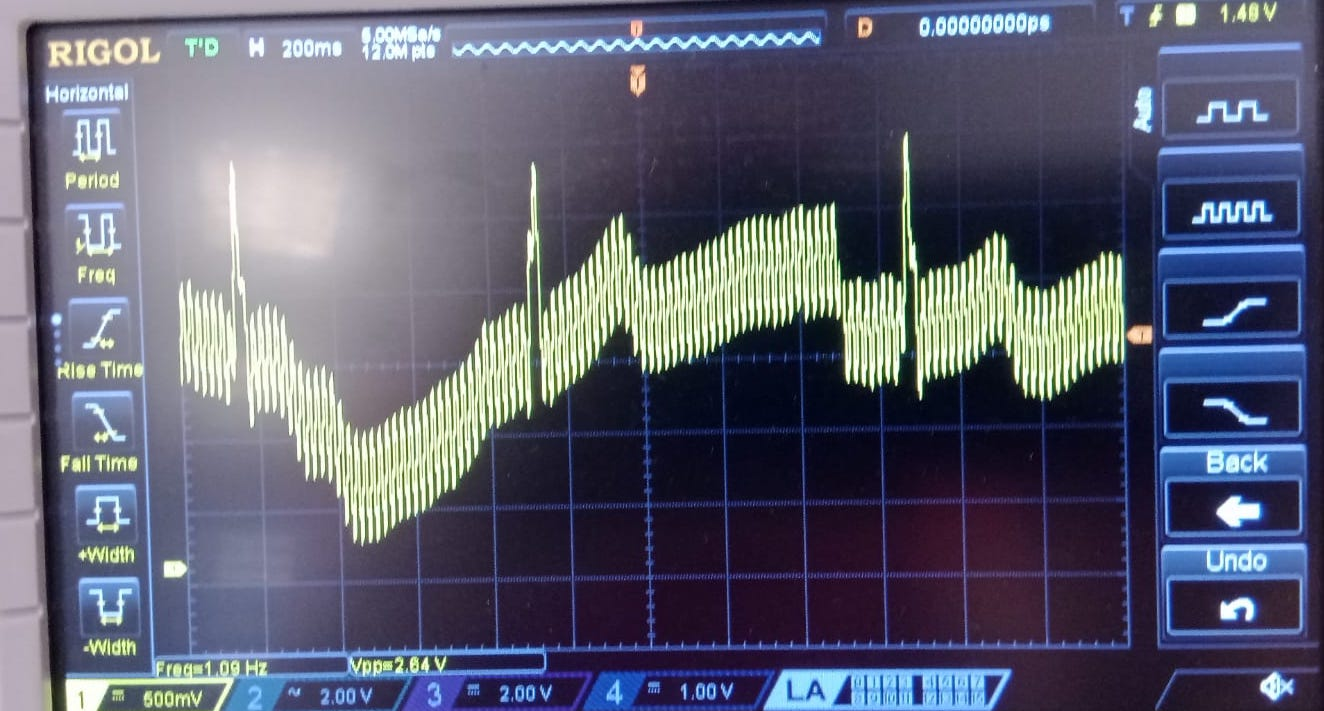
\includegraphics[width=0.45\textwidth]{d_SINelectrodo_SINnotch.jpg}}
    \caption{D.E. I sin tercer electrodo, sin filtro notch, manos en rodillas}
    \end{figure}
\begin{figure}[H]
    \centerline{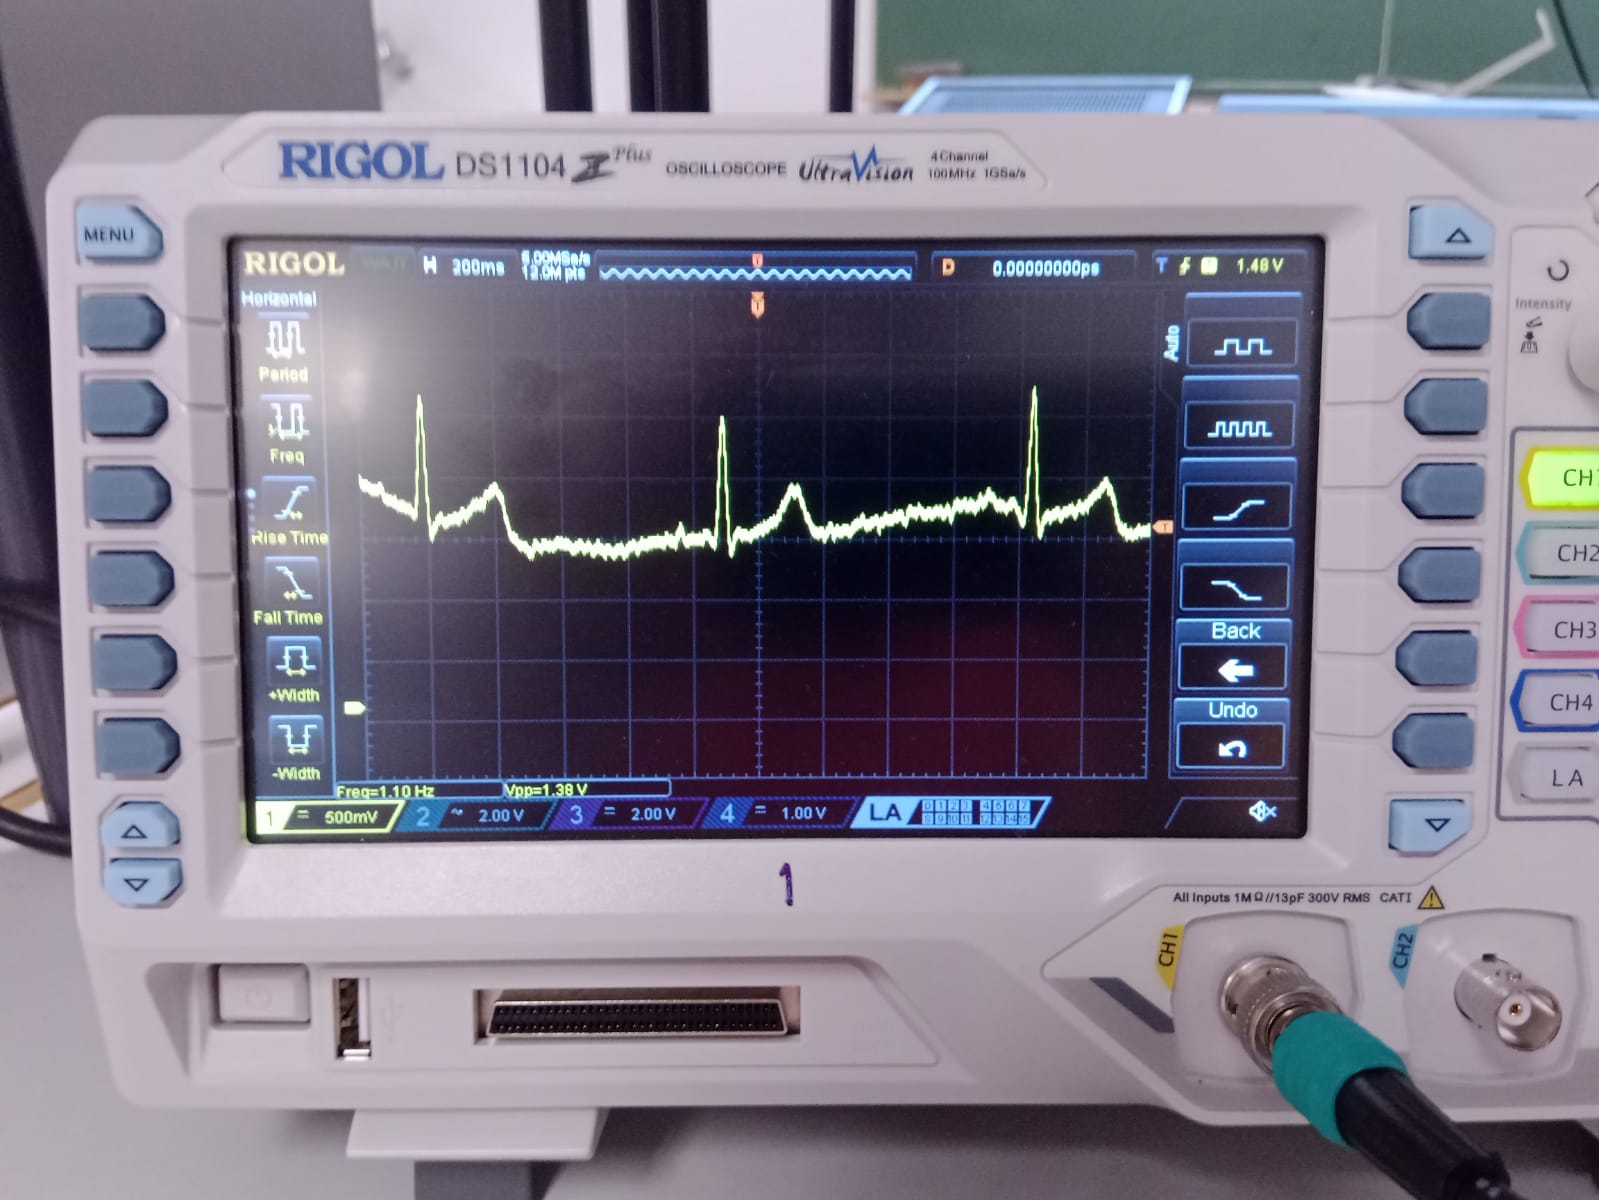
\includegraphics[width=0.45\textwidth]{d_SINelectrodo_CONnotch.jpg}}
    \caption{D.E. I sin tercer electrodo, con filtro notch, manos en rodillas}
    \end{figure}

\subsubsection{Mesa}
Al posicionar las manos sobre la mesa y al tener el filtro desconectado, la señal resultante resulta muy ruidosa como se observa en la siguiente figura.
\begin{figure}[H]
    \centerline{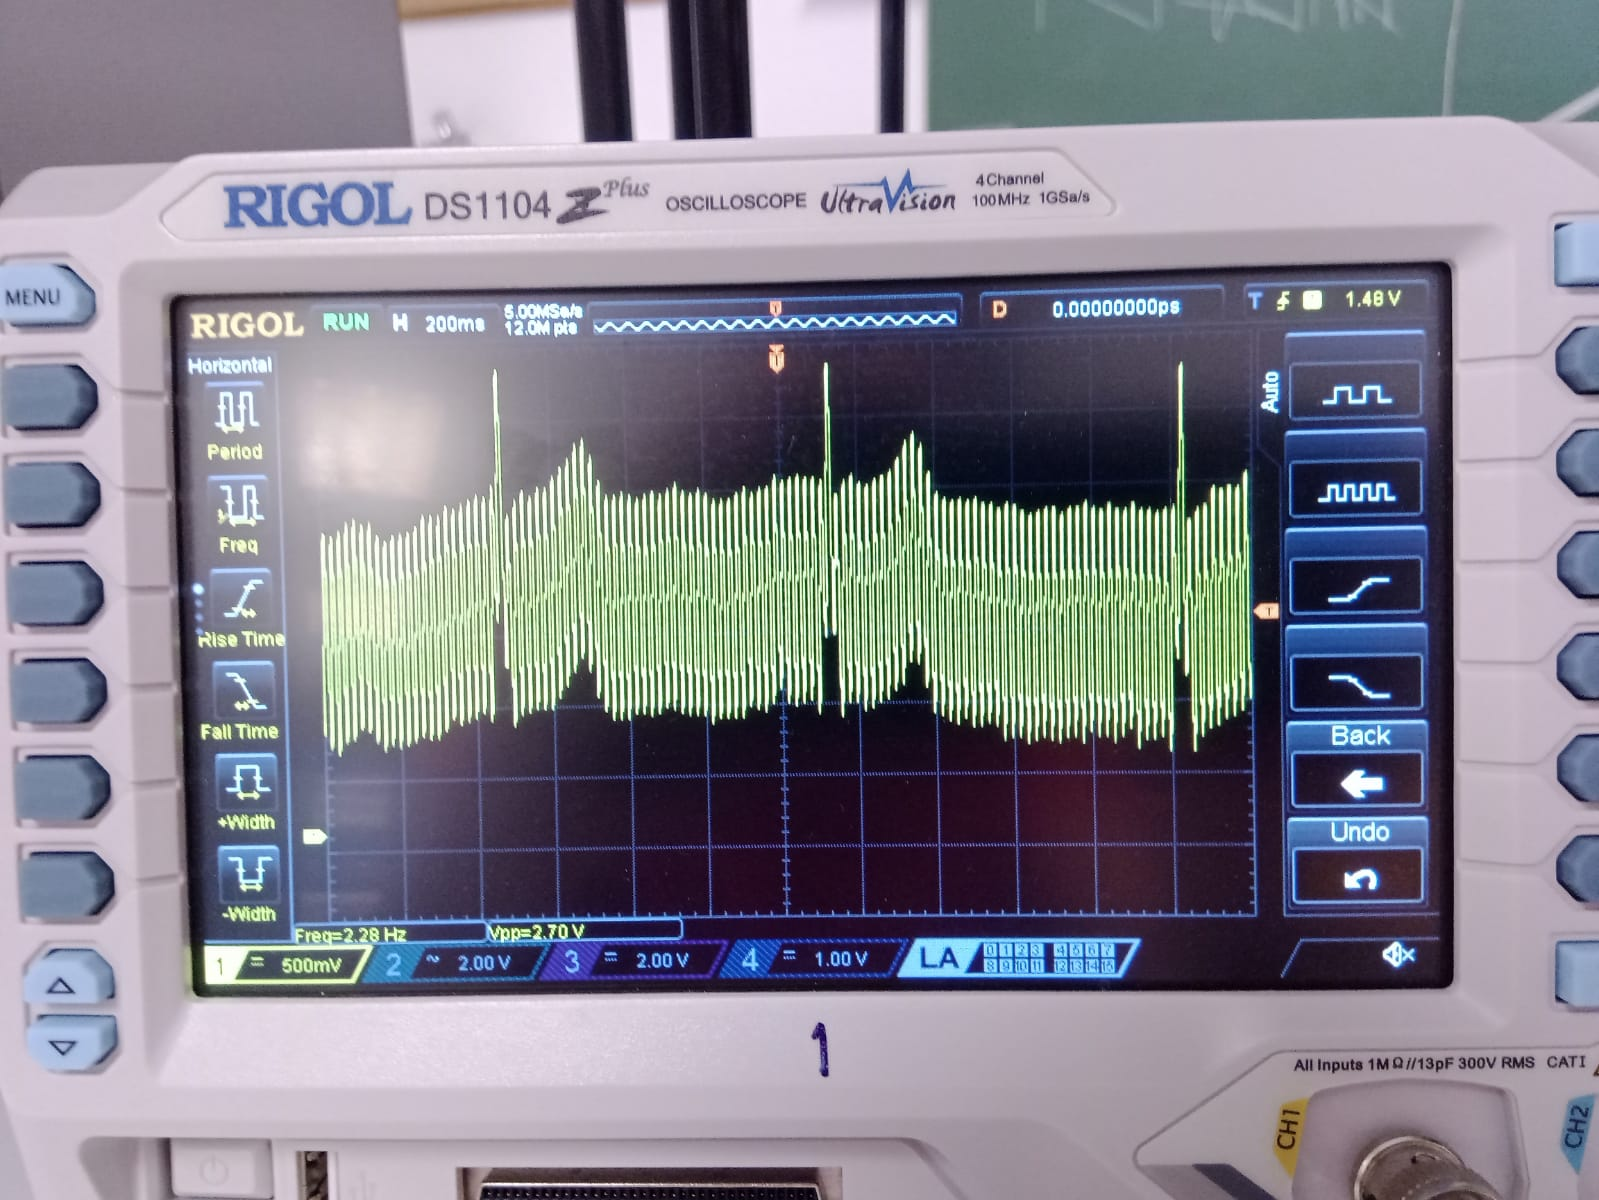
\includegraphics[width=0.45\textwidth]{d_SINelectrodo_SINnotch_mesa.jpg}}
    \caption{D.E. I sin tercer electrodo, sin filtro notch, manos en mesa}
    \end{figure}

\subsubsection{Aire}
Al dejar las manos en el aire y al tener el filtro desconectado, la señal sale ruidosa, aunque menos que si reposamos las manos sobre la mesa.
\begin{figure}[H]
    \centerline{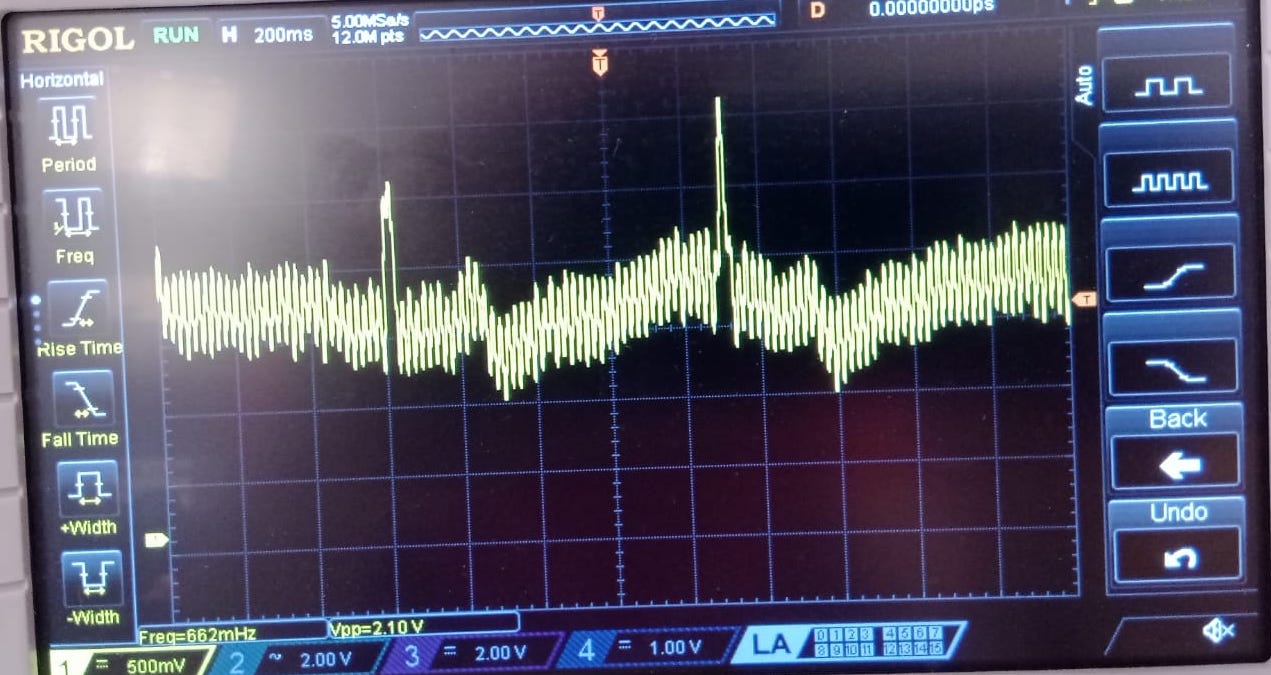
\includegraphics[width=0.45\textwidth]{d_SINelectrodo_SINnotch_aire.jpg}}
    \caption{D.E. I sin tercer electrodo, sin filtro notch, manos en el aire}
    \end{figure}

En los casos anteriores se estaba cerrando el circuito reposando la mano derecha sobre el conector del electrodo pero sin conectarlo. Ya que si no se cerraba el circuito haciendo contacto con éste último, la señal resultante sería nula, como se muestra en la siguiente imagen.
\begin{figure}[H]
    \centerline{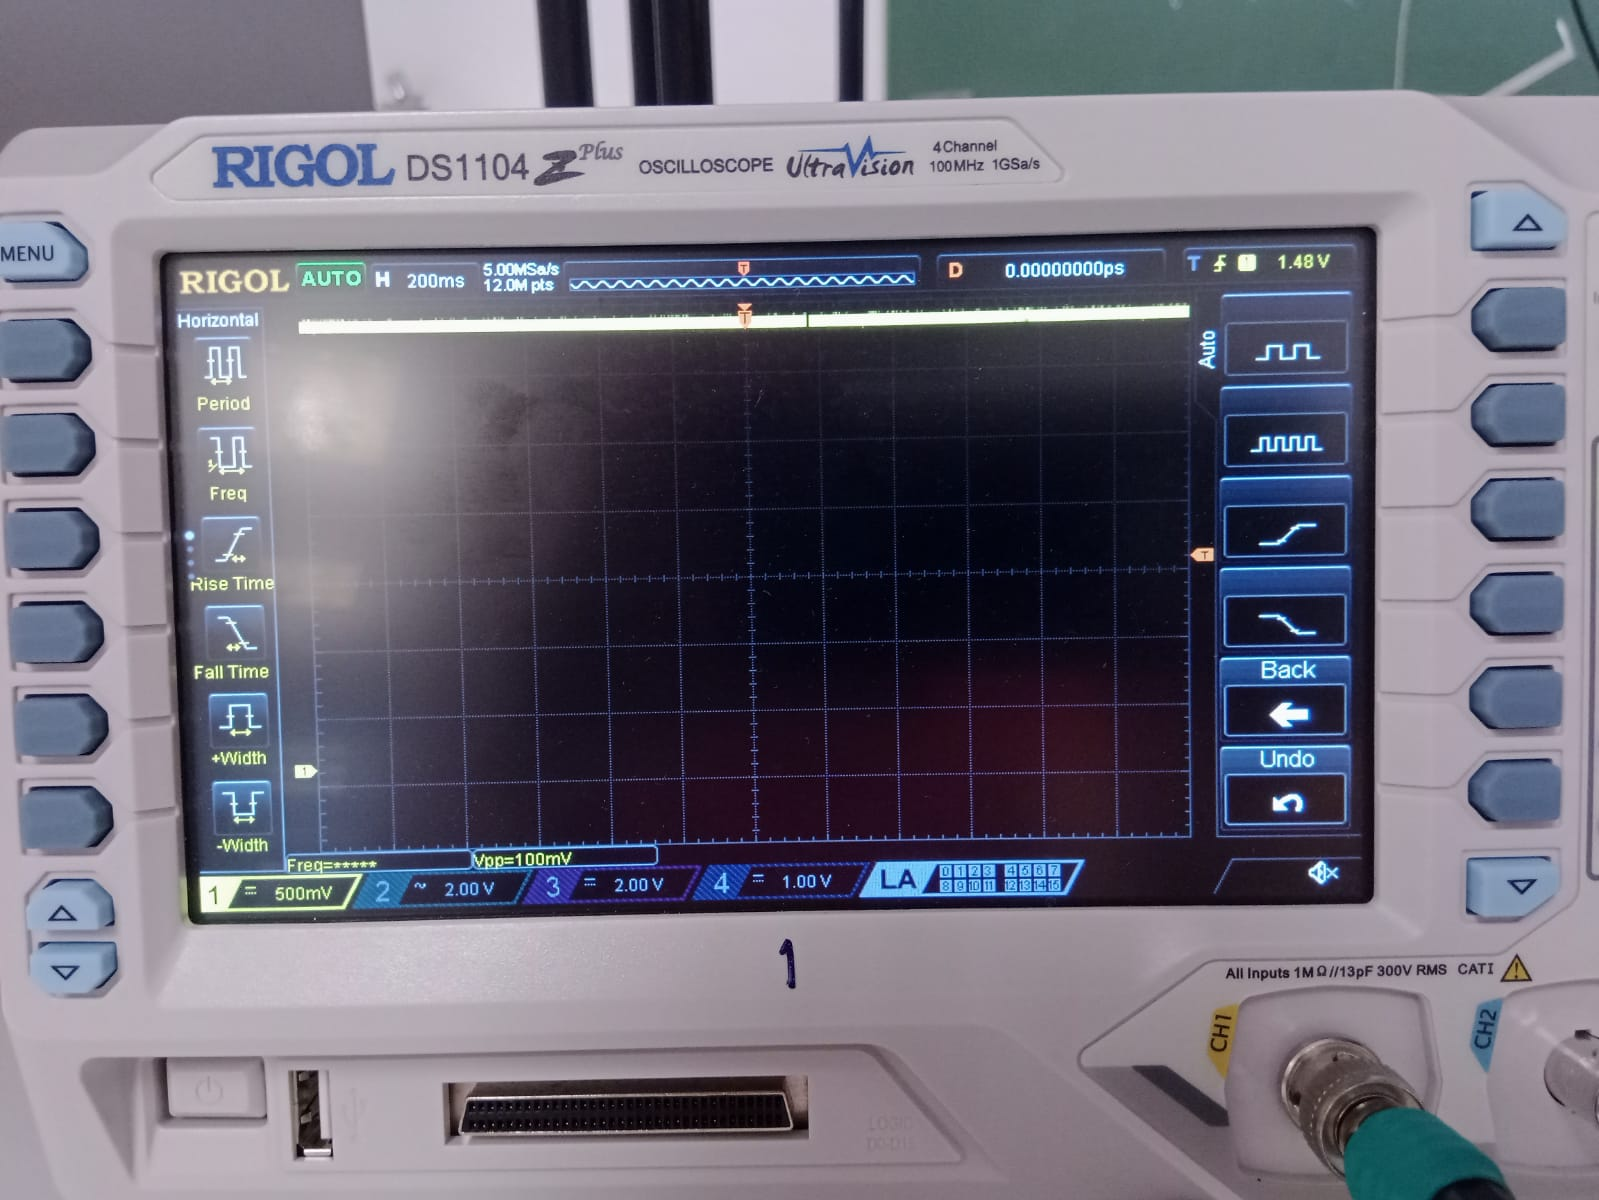
\includegraphics[width=0.45\textwidth]{d_SinElectrodo_sintocar.jpg}}
    \caption{D.E. I sin tercer electrodo, sin contacto}
    \end{figure}

\subsection{Derivación estándar I con tercer electrodo}
\subsubsection{Rodillas}
En las siguientes dos figuras se puede observar el funcionamiento de la señal con el tercer electrodo, se puede observar que la señal es algo más clara que si no utilizamos electrodo, pues la resistencia entre el conector y la piel es menor si se hace uso del electrodo.

Obviamente, si se pone en funcionamiento el filtro notch, la señal se ve sin el ruido que introduce la red eléctrica, como se observa en las dos imágenes que siguen.
\begin{figure}[H]
    \centerline{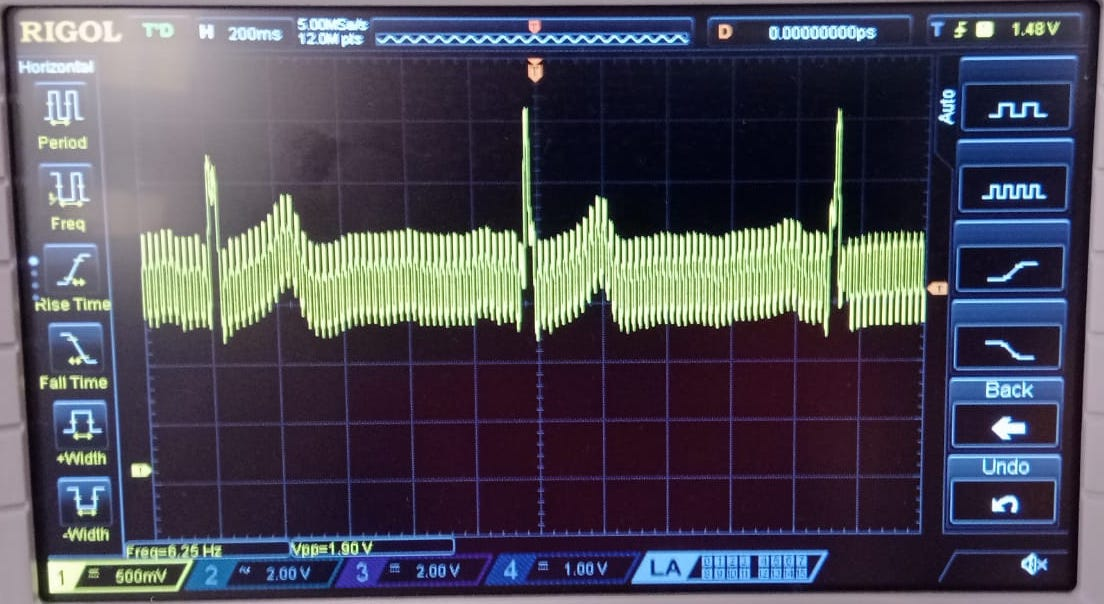
\includegraphics[width=0.45\textwidth]{d_CONelectrodo_SINnotch.jpg}}
    \caption{D.E. I con tercer electrodo, sin filtro notch, manos en rodillas}
    \end{figure}

\begin{figure}[H]
    \centerline{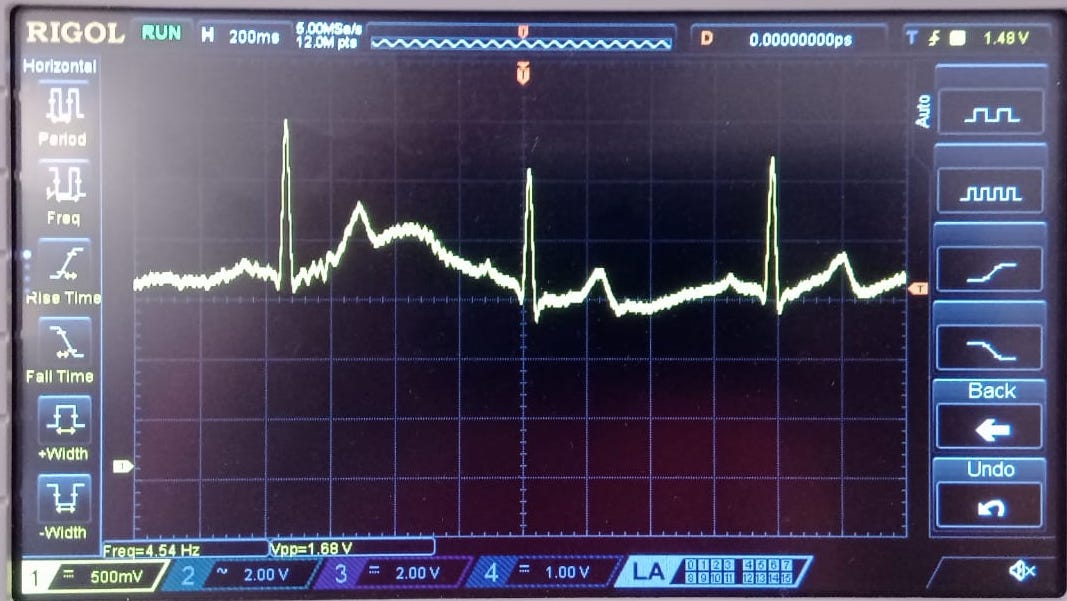
\includegraphics[width=0.45\textwidth]{d_CONelectrodo_CONnotch.jpg}}
    \caption{D.E. I con tercer electrodo, con filtro notch, manos en rodillas}
    \end{figure}

\subsubsection{Mesa}
En este caso, si posicionamos las manos sobre la mesa, se observa como se introduce algo de ruido aún teniendo conectado el filtro notch.
\begin{figure}[H]
	\centerline{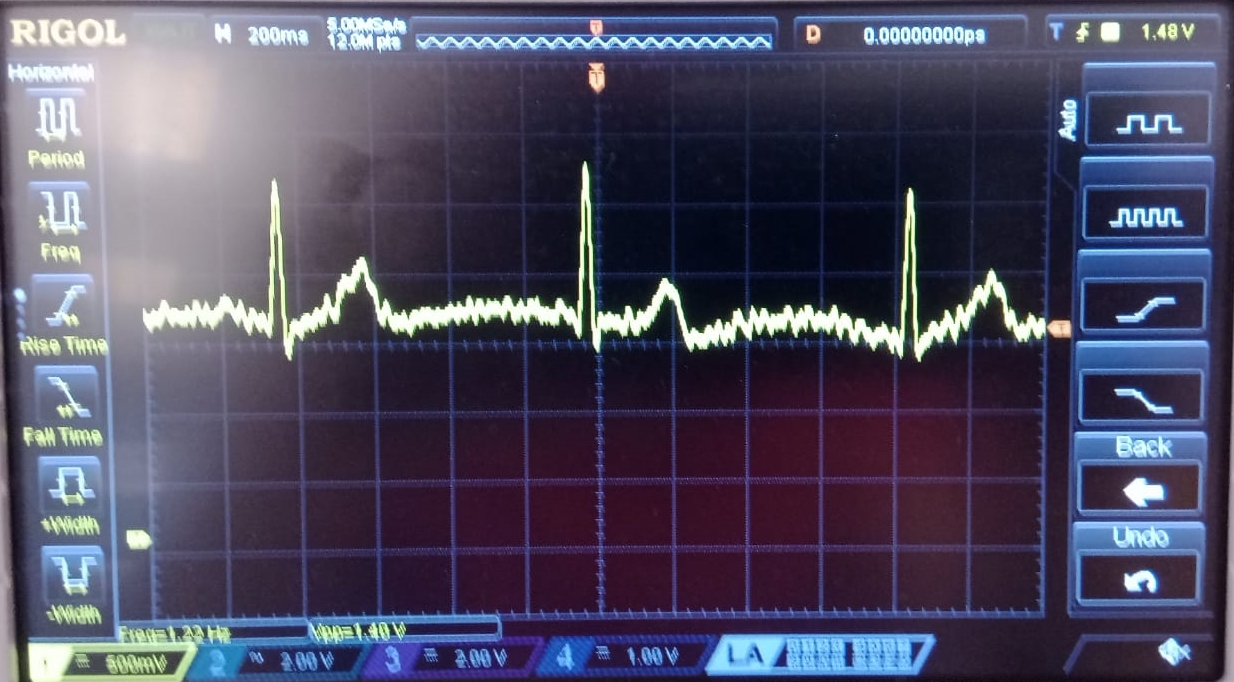
\includegraphics[width=0.45\textwidth]{d_CONelectrodoCONnotch_mesa}}
	\caption{D.E. I con tercer electrodo, con filtro notch, manos en la mesa}
	\end{figure}
    
\section{Sistema de adquisición de señales electrocardiográficas}
\subsection{Adquisición de derivaciones electrocardiográficas estándar}
En la siguiente imagen se puede observar el diagrama de bloques del VI, la parte que está resaltada es la que inicialmente nos aparecería en el programa.
\begin{figure}[H]
    \centerline{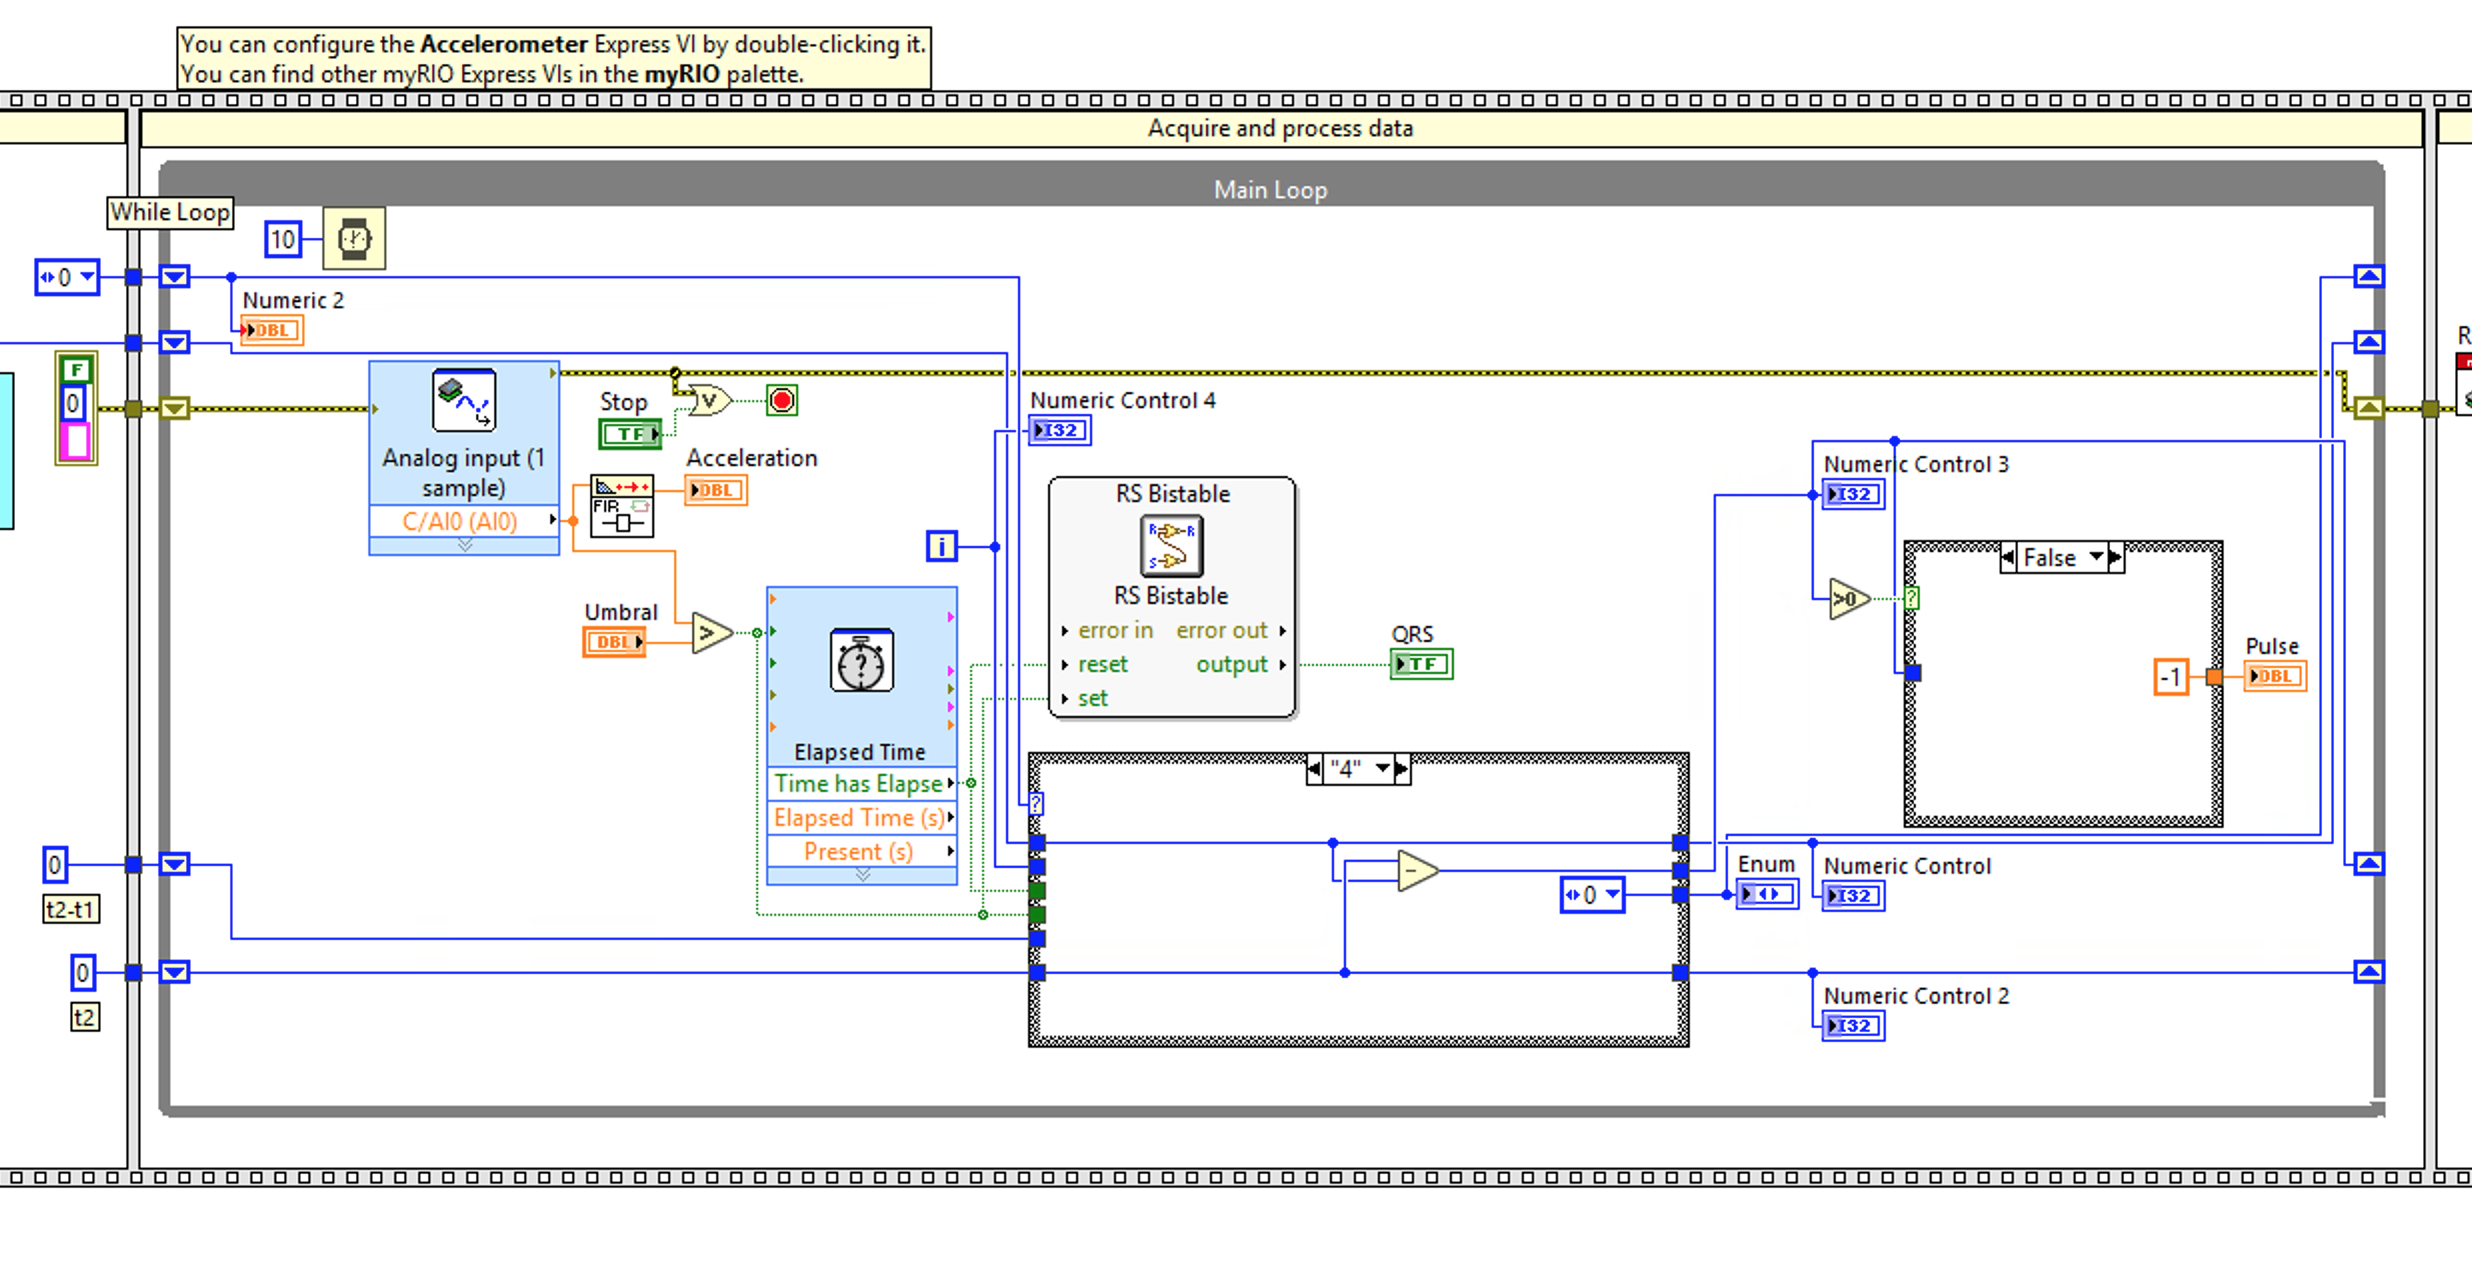
\includegraphics[width=0.45\textwidth]{e_diagramVI.png}}
    \caption{Block diagram VI inicial}
    \end{figure}

En la figura siguiente se muestra una captura de lo que es la Derivación Estándar I obtenida digitalmente mediante la myRIO y visualizada en LabVIEW.
\begin{figure}[H]
    \centerline{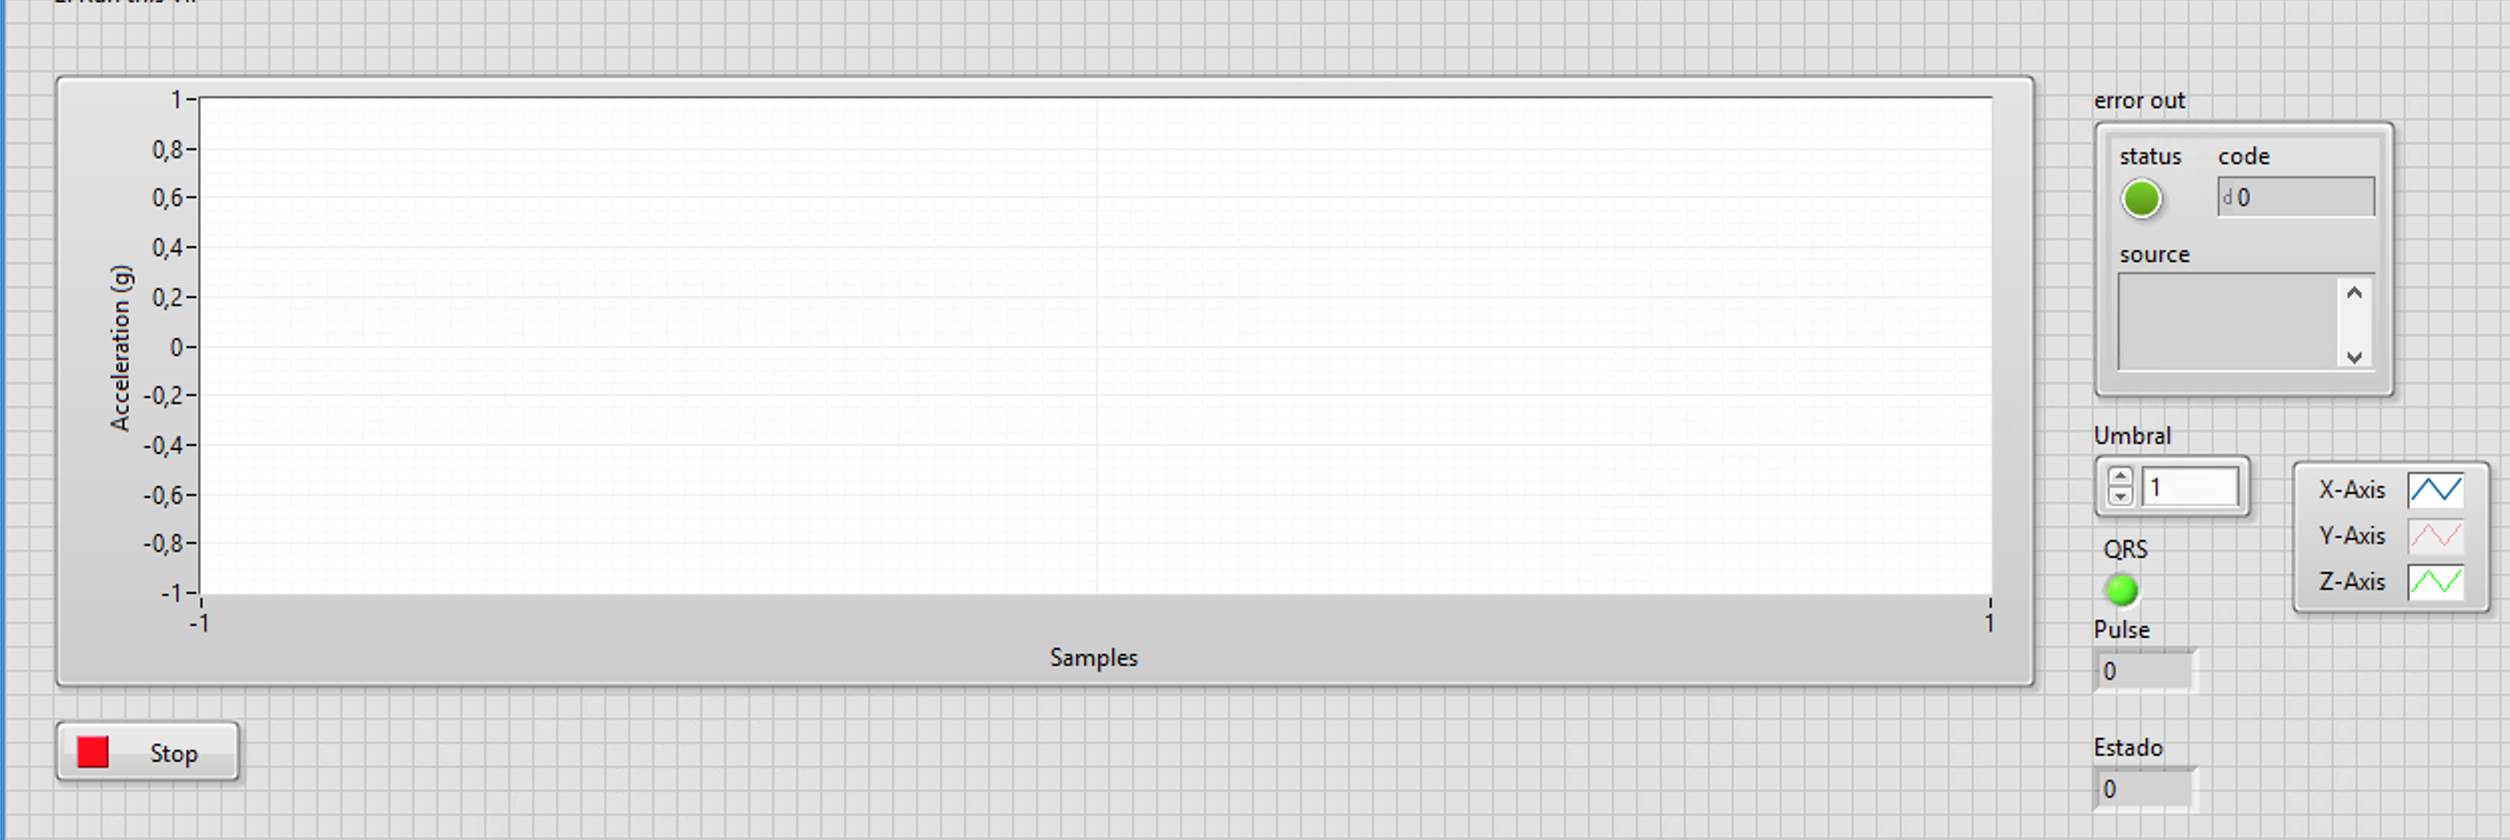
\includegraphics[width=0.45\textwidth]{e_captura.png}}
    \caption{Captura D. E. I en LabVIEW}
    \end{figure}

\subsection{Exportación de señales adquiridas}
Las 20 primeras líneas se adjuntan al final de este documento, son los valores fruto de la exportación de los datos a un documento Excel.
Y en la siguiente gráfica, se pueden ver los datos exportados representados:
\begin{figure}[H]
    \begin{tikzpicture}
        \begin{axis}[
            grid=both,
            xlabel={Muestra},
            ylabel={V (V)}]
        \addplot+[mark=none] table [x=x, y=y, col sep=comma] {g_myRIO.csv};
        \end{axis}
        \end{tikzpicture}
    \caption{Señal de la D. E. I, obtenida con myRIO}
    \label{g_myRIO}
    \end{figure}

\subsection{Detector de QRS digital}
Para mostrar cuando se mostraba un QRS en un instante concreto para así verlo gráficamente por un led, se programó de la siguiente manera en LabVIEW:
\begin{figure}[H]
    \centerline{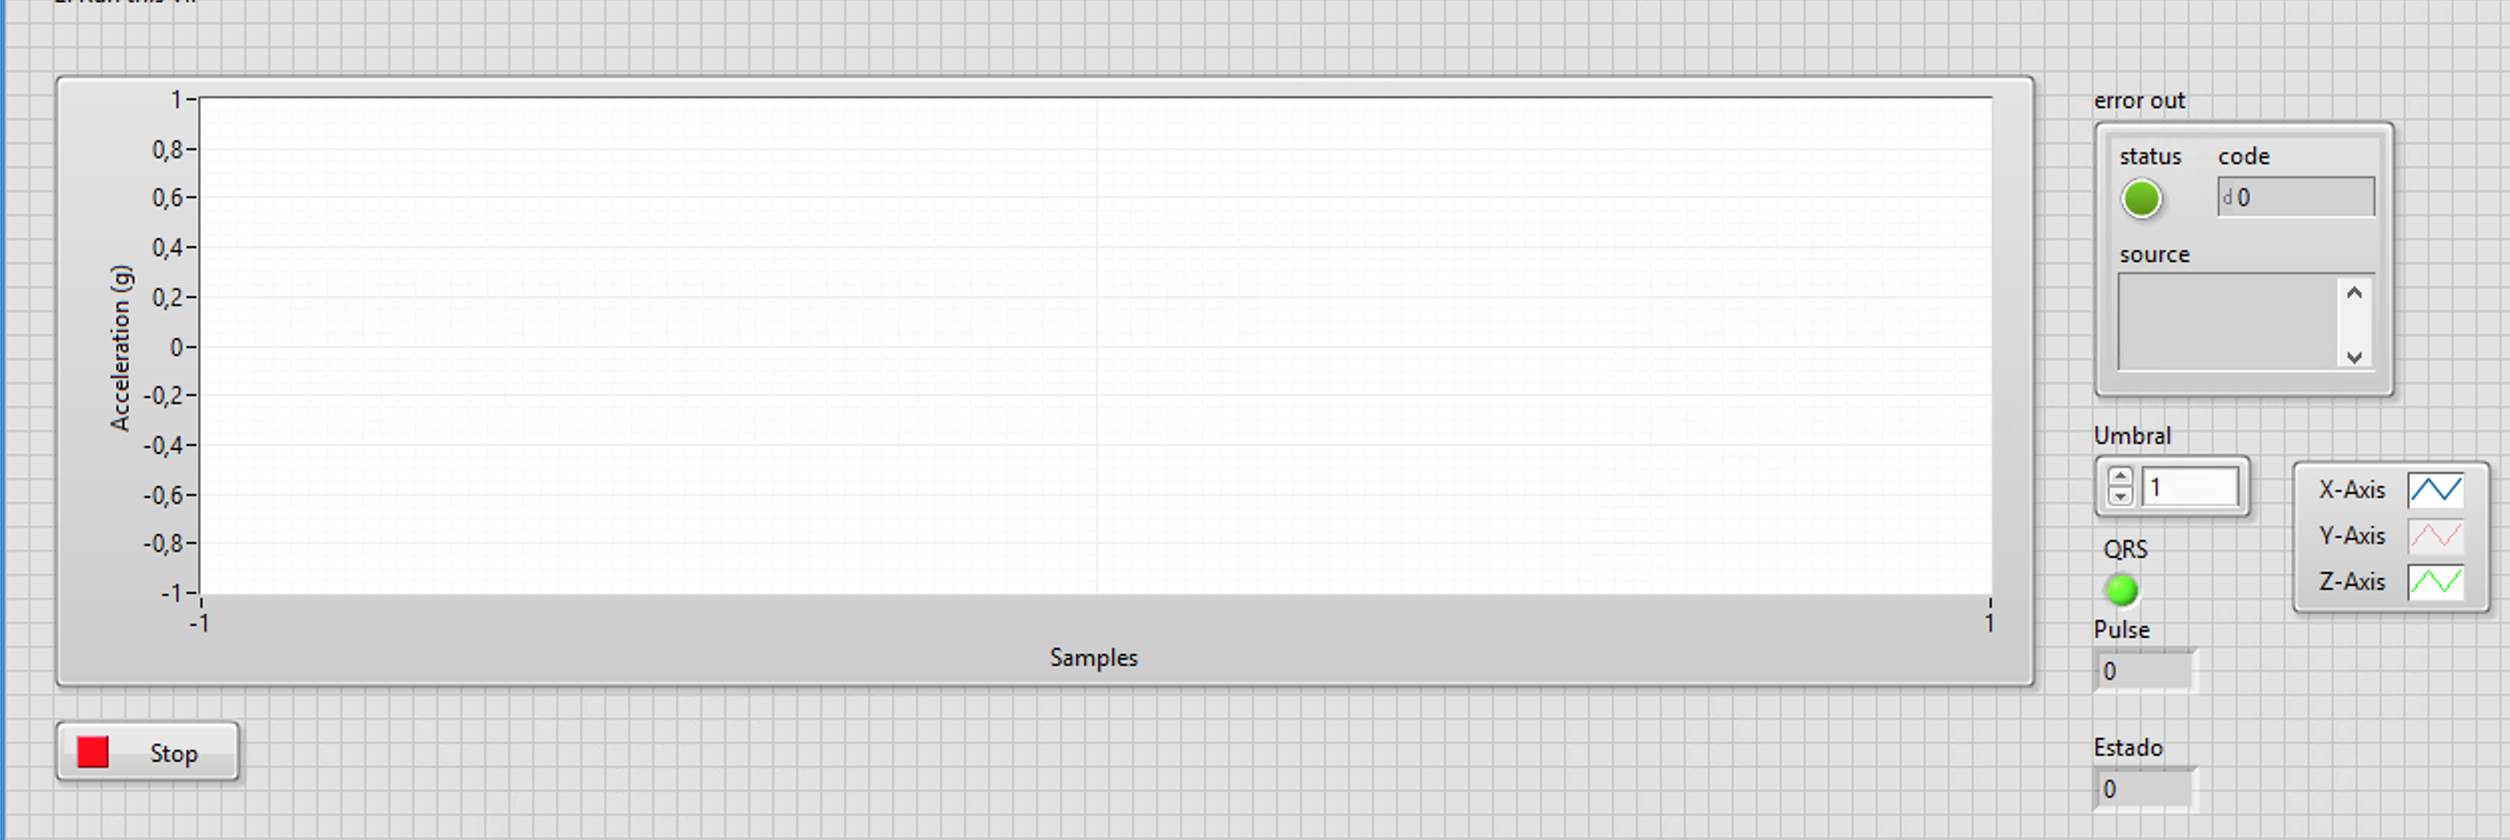
\includegraphics[width=0.45\textwidth]{e_captura.png}}
    \caption{Captura D. E. I en LabVIEW}
    \end{figure}

De manera que cuando la señal supera el nivel de umbral que le hemos configurado y que se puede modificar cuando el programa está en ejecución, se encienda un LED llamado QRS.

\subsection{Pulsómetro}
Utilizando la información que se nos proporciona, también podríamos saber las pulsaciones por minuto (bpm) sabiendo el intervalo de tiempo que hay entre dos picos del QRS. Haciendo la inversa y multiplicando por el factor oportuno se obtienen las pulsaciones por minuto.

Dado que no se estaba en el laboratorio cuando se terminó de diseñar este pulsómetro, se simuló el QRS mediante una señal cuadrada con un \textit{duty-cycle} de un 10\% y la misma frecuencia que la que tendría la señal original. Aún así, el resultado sigue siendo óptimo.
\begin{figure}[H]
    \centerline{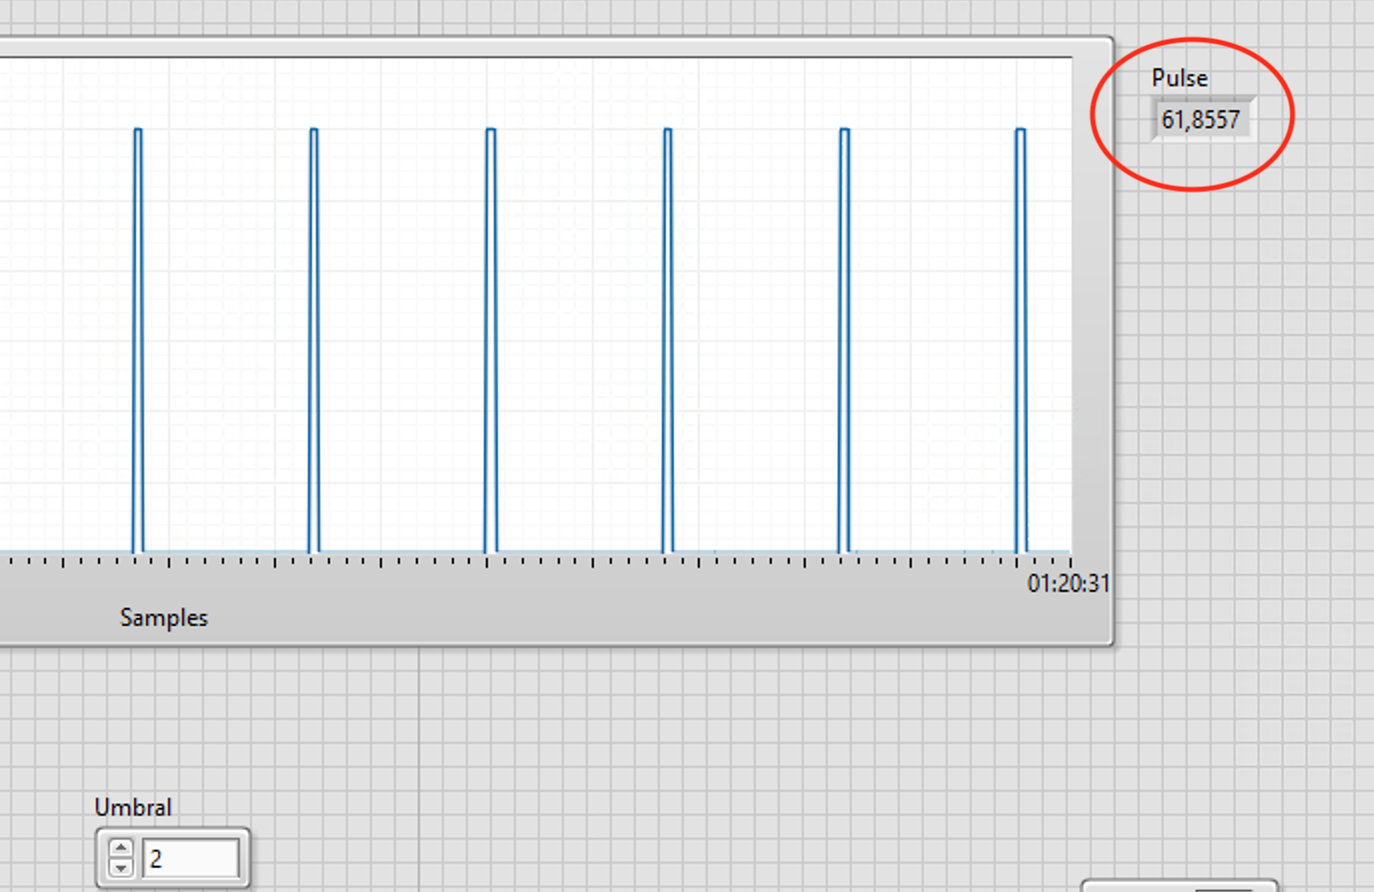
\includegraphics[width=0.45\textwidth]{e_pulsometro.png}}
    \caption{Pulsómetro en LabVIEW}
    \end{figure}


\begin{table}[H]
\caption{20 primeras líneas del archivo de datos exportado}
\begin{center}
	\begin{tabular}
	\hline
	\textbf{Samples - X-Axis} & \textbf{Acceleration (g) - X-Axis} \\ \hline
	979                       & 157715,00                          \\ \hline
	980                       & 151367,00                          \\ \hline
	981                       & 145996,00                          \\ \hline
	982                       & 145020,00                          \\ \hline
	983                       & 146484,00                          \\ \hline
	984                       & 146484,00                          \\ \hline
	985                       & 147461,00                          \\ \hline
	986                       & 149902,00                          \\ \hline
	987                       & 153809,00                          \\ \hline
	988                       & 154785,00                          \\ \hline
	989                       & 151855,00                          \\ \hline
	990                       & 148438,00                          \\ \hline
	991                       & 148926,00                          \\ \hline
	992                       & 150391,00                          \\ \hline
	993                       & 150391,00                          \\ \hline
	994                       & 150879,00                          \\ \hline
	995                       & 151367,00                          \\ \hline
	996                       & 151367,00                          \\ \hline
	997                       & 151855,00                          \\ \hline
\end{tabular}
\end{center}
\end{table}
\end{document}
